% ===========================================================================
% Section IV-A -- Filter Architecture and Pole-Zero Stability Analysis
% Owner: Member 2
% ===========================================================================
\subsection{Filter Architecture and Pole--Zero Stability Analysis}
The Kurtogram was run on the pre-processed $12$~kHz record. Over the levels
spanning $[0, 6000]$~Hz it chose a band centered at $f_c^* = 3000.0$~Hz with
$BW^* = 2000.0$~Hz, which puts the cutoffs at $2000.0$~Hz and $4000.0$~Hz.
Inside that band the kurtosis peaked at $K = 4.58$. The broadband input sat at
$K = 2.23$.

\begin{figure*}[!t]
\centering
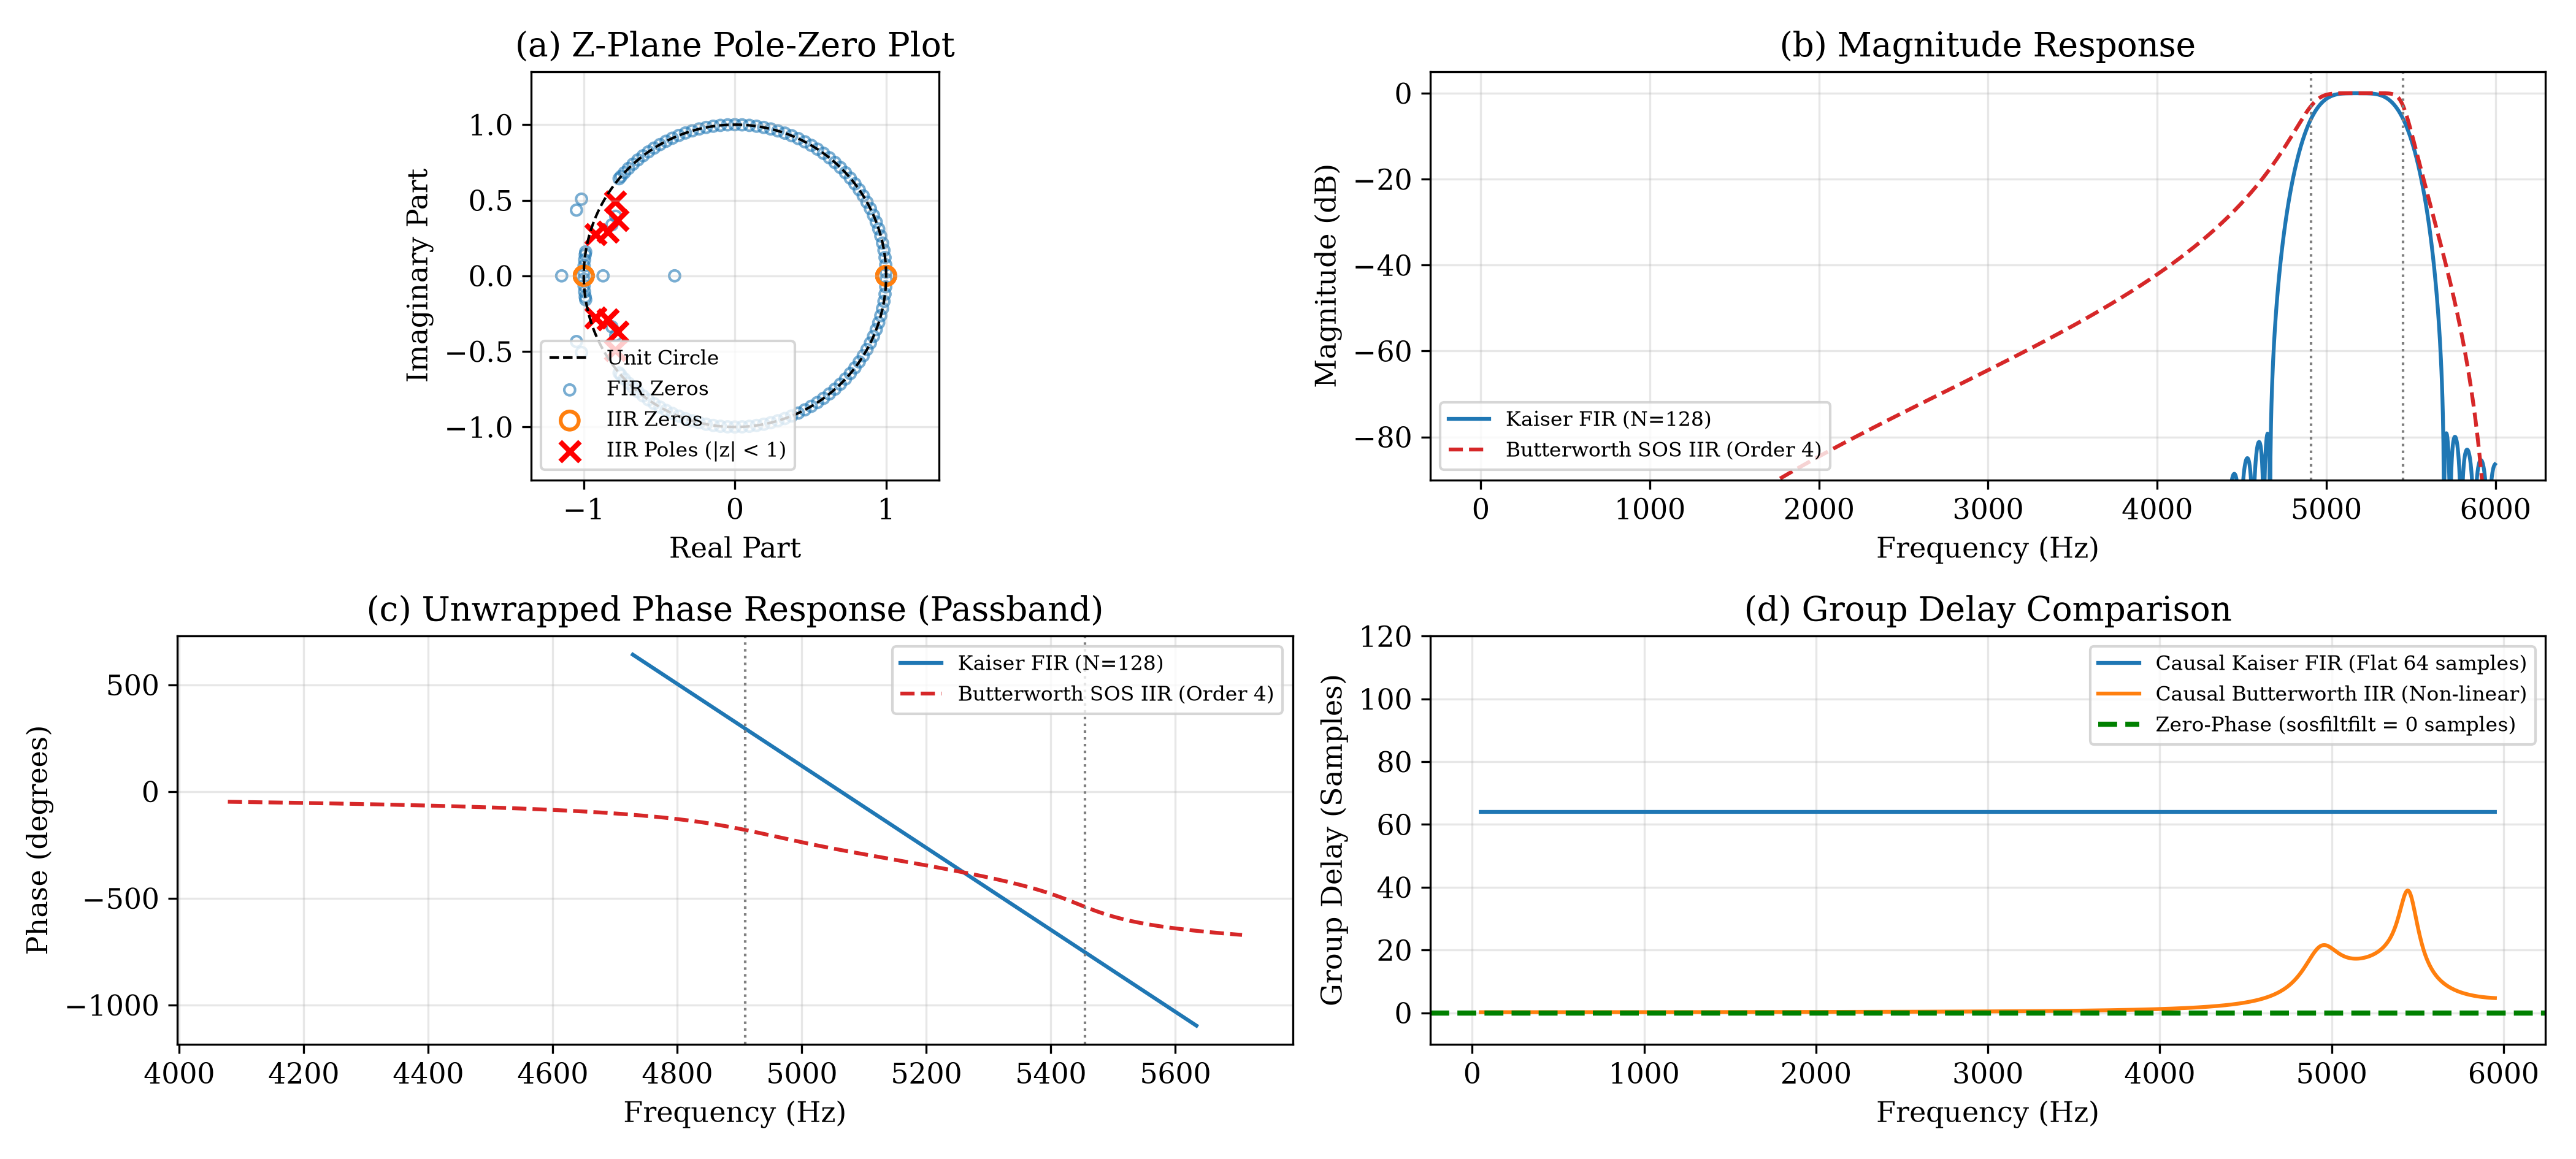
\includegraphics[width=0.98\textwidth]{Fig1_Filter_PoleZero_Comparison.png}
\caption{Comparison of the Type-I Kaiser-windowed FIR bandpass filter
($M = 128$, $129$~taps, $\beta = 8.0$) and the $4^{\text{th}}$-order
Butterworth Cascade SOS IIR bandpass filter across the Kurtosis-selected
passband $[2000, 4000]$~Hz: (a) complex $z$-plane pole--zero plot verifying that
all IIR poles lie strictly inside the unit circle ($r_{\max} = 0.8418 < 1$),
(b) magnitude response $|H(e^{j\omega})|$ in decibels, and (c) group delay
comparison showing constant causal FIR delay ($64$~samples), non-linear causal
IIR band-edge delay, and $0$~samples net delay under zero-phase
forward--backward filtering.}
\label{fig:filter_comparison}
\end{figure*}

With the band fixed, a Type-I Kaiser FIR ($M = 128$, $L = 129$~taps,
$\beta = 8.0$) was compared against a $4^{\text{th}}$-order Butterworth IIR in
cascade SOS form (four biquads). Fig.~\ref{fig:filter_comparison} shows the
pole--zero map, the magnitude response and the group delay.

In Fig.~\ref{fig:filter_comparison}(a) the FIR has zeros spread along the
stopband arcs and every pole at the origin. The IIR is different. The bilinear
transform puts four zeros at $z = 1$, which blocks DC, and four at $z = -1$,
which blocks Nyquist, with four conjugate pole pairs inside the passband arc.
Its largest pole radius is $r_{\max} = 0.8418$. The region of convergence
$|z| > 0.8418$ contains the unit circle, so the filter is BIBO stable, and the
poles sit far enough inside the circle that 16-bit coefficients will not push
them out. The four zeros at $z = \pm1$ are exact nulls rather than deep
attenuation, which is why DC and Nyquist are blocked completely.

Fig.~\ref{fig:filter_comparison}(b) compares magnitudes. Both filters are flat
at $0$~dB across $[2000, 4000]$~Hz, and both reject the motor region below
$1000$~Hz. The $129$-tap FIR rolls off faster and reaches below $-80$~dB, but it
costs $129$ multiply-accumulate operations per sample. The four-section SOS
filter needs $4 \times 5 = 20$, which is $84\%$ fewer.

Fig.~\ref{fig:filter_comparison}(c) is the group delay. In causal operation the
FIR delays every frequency by the same $64$ samples. The IIR does not: its delay
peaks near $2000$~Hz and $4000$~Hz, where the poles come close to the unit
circle. With forward--backward filtering the effective response is
$|H(e^{j\omega})|^2$, the phase term cancels, and the delay is zero samples
everywhere.
